\section{Motivation} \label{sec:motivation}
In this section, we take our own experience on optimizing BFS 
with Xilinx HLS as an example and exhibit the design challenge. Then we will 
evaluate the irregular memory access efficiency and show its influence 
on BFS performance when implemented with OpenCL.

\subsection{High level synthesis optimization challenge}
High level synthesis tools greatly alleviate the efforts of building BFS accelerators on FPGAs. 
Nevertheless, the performance of the resulting accelerators can be far from satisfying 
especially for irregular applications like BFS. In this section, we take our own experience 
on optimizing BFS on Alpha-Data as an example and show the challenge of 
optimizing BFS with HLS tools.

We started from basic sequential BFS algorithm for 
the HLS design. First of all, we separated the nested loop into different pipeline 
stages connected via FIFO using data flow model supported by Xilinx HLS. 
We explored all the possible pipeline combinations ranging from single-stage 
pipeline to seven-stage pipeline. With the optimized pipeline, we further 
introduced prefetch buffer to improve memory access efficiency, 
added customized cache structure for the vertex property to reduce the external 
memory accesses, hash table based redundancy removal logic to reduce the repeated 
outgoing neighboring vertices of the frontier vertices. Finally, we also tried to 
duplicate the pipeline stages for parallel processing and tuned the design parameters 
of the accelerators such as cache and prefetch buffer size. We believed 
we had tried the major design optimization methods that could be applied to the 
baseline HLS design. 

%\begin{algorithm}
%	\caption{BFS Algorithm} \label{alg:bfs}
%    \small
%	\begin{algorithmic}[1]
%		\Procedure{BFS}{}
%		\State $level[v_k] \gets -1$ where $v_k \in V$
%		\State $level[v_s] \gets 0$
%		\State $current\_level \gets 0$
%		\State $frontier \gets v_s$
%
%        \While {$!frontier.empty()$} 
%
%		\For{$v \in V$}
%		\If{$level[v] == current\_level$}
%		\State $frontier \gets v$
%		\EndIf
%		\EndFor
%
%		\For{$v \in frontier$}
%		\State $S \gets {n \in V | (v, n) \in E}$
%		\For {$n \in S$}
%		\If {$level[n] == -1$}
%		\State $level[n] \gets current\_level + 1$
%		\EndIf
%		\EndFor
%		\EndFor
%		\State $current\_level \gets current\_level + 1$
%		\EndWhile
%		\EndProcedure
%	\end{algorithmic}
%\end{algorithm}

We measured the performance of the accelerator with a set of representative graphs 
including Youtube (YT), Live Journal(LJ), Pokec(PK) and two R-MAT graphs. Details about the 
graph benchmark can be found in Table \ref{tab:graph} in the experiment section. 
Figure \ref{fig:opt-performance} presents the normalized performance
when different optimization techniques are gradually applied to the naive baseline design.
It can be found that the resulting BFS accelerator achieves up to 70X performance speedup
compared to the baseline design. While the basic optimizations can improve the BFS
performance significantly, it is still far from ideal compared to the state-of-art 
handcrafted design on FPGAs \cite{betkaoui2012reconfigurable}, 
\cite{attia2014cygraph}, \cite{zhang2017boosting}, \cite{nurvitadhi2014graphgen},
\cite{dai2016fpgp}. Therefore, the current BFS needs a careful redesign to achieve 
competitive performance. This motivates us to study the bottleneck of 
the baseline implementation and to develop new design with OpenCL.

\begin{figure}
	\center{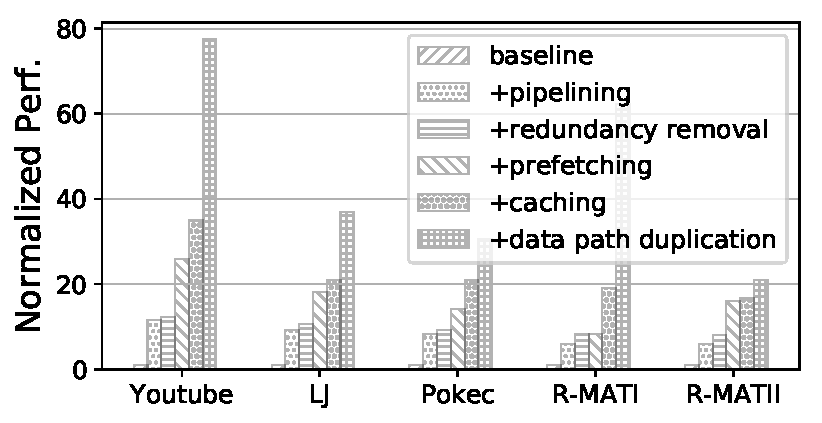
\includegraphics[width=0.8\linewidth]{opt-performance}}
    \caption{The normalized performance of an HLS based BFS accelerator with various optimizations on Alpha-Data}
\label{fig:opt-performance}
\vspace{-1em}
\end{figure}

%While the baseline design could be created using HLS in around an hour, optimizing the 
%HLS design took much longer time. 
Another challenge of the BFS design with HLS is the optimization productivity. 
The optimization took an experienced hardware designer 
with basic high level synthesis knowledge up to months, though most of time was 
spent on implementing the large amount of combined optimization methods and cumbersome
debugging when software simulation passed but the accelerator got stalled 
during hardware execution. This motivates us to focus on the high-level BFS 
accelerator optimization and offer open-sourced BFS design with both 
the near handcrafted performance and the software-like flexibility.
 
%accelerator using HLS tools remains a challenging task and will be even more difficult for 
%designers without much hardware knowledge. Meanwhile, we also notice that the benefits of 
%the HLS design is also attractive. Despite the difference between Xilinx HLS 
%and Intel OpenCL, porting the design to FPGA devices of different vendors is trivial. 

%Therefore, we argue that it is beneficial to have the experienced designers to explore the HLS based 
%application acceleration and provide the HLS solutions to more users without hardware 
%experiences. This motivates us to focus on the high-level BFS accelerator optimization
%and offer open-sourced BFS design with both the near handcrafted performance and 
%the software-like flexibility.

\subsection{Inefficient irregular memory access}
As discussed in Section \ref{sec:intro}, there are large amount of irregular memory access in BFS, 
but it is non-trivial to evaluate its influence on BFS performance directly. To gain in-depth 
analysis of the irregular memory access in BFS with OpenCL, we present two different experiments.

In this first experiment, we measured the irregular memory access latency on Intel Harp-v2.
Three typical memory access patterns including sequential memory access, dependent random memory access 
and independent random memory access are presented. Note that dependent random memory access 
means that the random access is dependent and they must be handled sequentially while the independent random 
access allows the requests to be processed in parallel. Both random access patterns appear in OpenCL based BFS.
Particularly, many independent memory access may be taken as dependent memory access in BFS because the 
OpenCL compiler has no algorithm-specific information. Data width is also critical to the memory access 
when implemented in OpenCL, different data width are 
analyzed as well. 

The experiment result is shown in Figure \ref{fig:avg-mem-lat}. It can be found that independent memory 
access leads to orders of magnitude of higher latency. Data width is critical to all the memory access patterns.
While dependent memory access efficiency increasingly improves with the data width, dependent memory access and sequential memory 
access efficiency gets saturated when the data width reaches 1024 bit and 512 bit respectively. According to the experiment, 
we should avoid potential memory conflict in OpenCL where the compiler will take them as dependent and generate 
dependent memory access requests. Also the designers should try to access memory with larger aligned data width. 
\begin{figure}
	\center{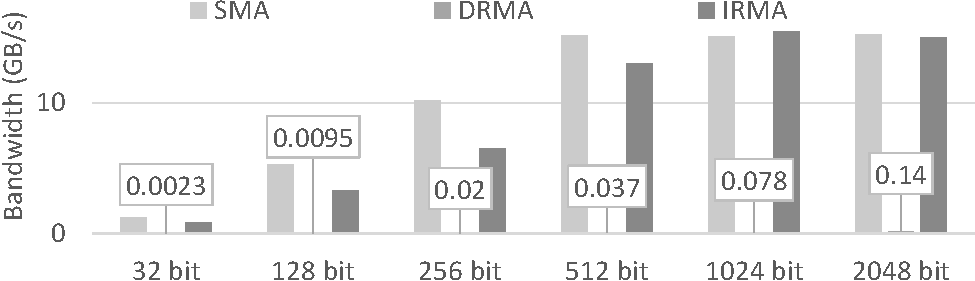
\includegraphics[width=0.85\linewidth]{avg-mem-lat}}
    \caption{Normalized average memory access latency per byte. Note that the latency is normalized to the 
	lowest latency of sequential memory access}
\label{fig:avg-mem-lat}
\vspace{-0.5em}
\end{figure}


In the second experiment, we analyzed the distribution of the irregular memory access in BFS. 
When the burst size of a memory request is less than 4, we will classify 
it as irregular memory access. Note that the short burst memory access can also be considered as 
a random memory access with larger data width. As the starting vertex also affects the distribution, 
we calculated  the average percentage of 64 non-trivial BFS with random starting vertex. 
According to the experiment result on the five graphs 
in Figure \ref{fig:bfs-mem-dist}, we find that the majority of the memory access in BFS is irregular, 
though the amount of the irregular memory access takes up only a small portion of the total memory access. 
Since the irregular memory access latency may even be orders of magnitude higher 
especially for the dependent random memory access, the irregular memory access that is over 15\% of 
the total amount of memory access affects the BFS performance dramatically if it is not 
optimized appropriately. 
\begin{figure}
	\center{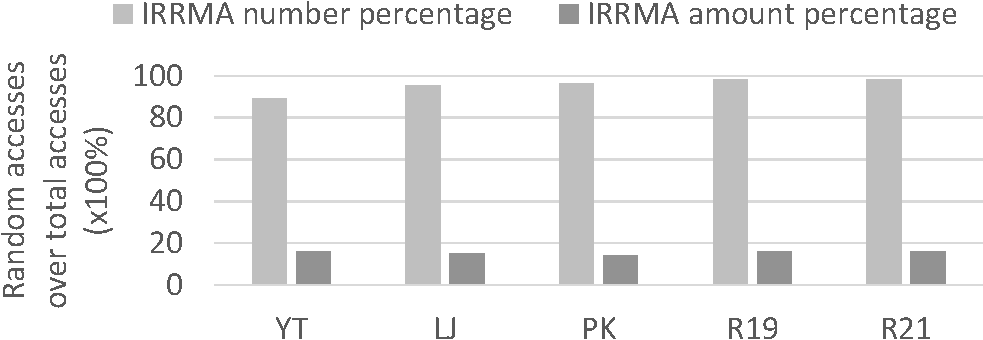
\includegraphics[width=0.85\linewidth]{bfs-mem-dist}}
    \caption{BFS iregular memory access distribution analysis. The amount of memory access refers to the amount of 
	bytes of the memory access while the number of memory access focuses on the number of memory requests.}
\label{fig:bfs-mem-dist}
\vspace{-0.5em}
\end{figure}


